\documentclass[10pt, a4paper]{aqademic}

\usepackage[spanish]{babel}
	\selectlanguage{spanish}

% Document packages

\usepackage{amsmath}
\usepackage[type=CC, modifier=by-nc-sa, version=4.0]{doclicense}
\usepackage{tikz}
	\usetikzlibrary{arrows,automata}

% Document settings

\author{Atanasio José Rubio Gil}
\title{Modelos de computación}

\AqSetChapter{Problema}

% Document composition

\begin{document}

\AqMaketitle[%
	cover    = logo-ugr.png,
	org      = Grado en Ingeniería Informática,
	subtitle = Problemas,
	url      = https://github.com/Groctel/ugr-informatica
]

\begin{titlepage}

\newgeometry{%
	left=5cm,
	right=5cm
}

\thispagestyle{empty}

\topskip0pt
\vspace*{\fill}

\begin{center}
	\textbf{\Huge{¡Gracias por apostar por el conocimiento libre!}}
\end{center}

\vspace{1cm}

Estos apuntes están compartidos libremente para que puedas estudiar de forma gratuita y sin bloques de publicidad molesta en tus páginas.
Su publicación y uso son un paso adelante en la idea de que el conocimiento debería ser compartido de forma libre y gratuita para todos sin ningún tipo de impedimentos o distracciones generadas por muros de pago.

Como autor, no recibo ningún tipo de ingreso por la confección y publicación de este material.
Si quieres colaborar y ayudarme a seguir ofreciéndote facilidades para estudiar, puedes unirte al proyecto a través del enlace de la portada o enviarme una propina mediante el siguiente botón o su enlace:

\vspace{0.5cm}

\begin{center}
	\href{https://ko-fi.com/groctel}{
\includegraphics[scale=0.15]{RecursosTeX/BuyMeACoffee_blue-2x.pdf}}
	\url{https://ko-fi.com/groctel}
\end{center}

\vspace{0.5cm}

Dado que este documento está compartido bajo una licencia \textbf{CC-by-nc-sa}, tienes la libertad de distribuirlo y adaptarlo bajo las siguientes condiciones:

\begin{itemize}
	\item\textbf{BY:} Debes darme crédito de forma adecuada con un enlace a la licencia e indicar si has hecho cambios.
	\item\textbf{NC:} No puedes hacer uso del mismo con propósitos comerciales.
	\item\textbf{SA:} Debes distribuir tus modificaciones bajo la misma licencia que el documento original.
\end{itemize}

Puedes leer la licencia completa pinchando en el enlace de la portada.

\vspace*{\fill}

\end{titlepage}

\tableofcontents

\chapter{}

\section{Enunciado}

Obtener la gramática para el lenguaje de palíndromos de orden par.

\section{Solución}

Para que las palabras sean de longitud par, vamos a crear reglas de producción que generen un carácter a ambos lados del único símbolo no terminal, de forma que la palabra se genere ``de dentro hacia fuera'' y sólo sustituir el símbolo no terminal por la regla anteriormente descrita y por la cadena vacía.

\begin{align*}
	G &= (V, T, P, S) : \\
	V &= \{E\} \\
	T &= \{a, b, c, d, e\} \\
	P &=
		\begin{cases}
			E \rightarrow aEa      \\
			E \rightarrow bEb      \\
			E \rightarrow cEc      \\
			E \rightarrow dEd      \\
			E \rightarrow eEe      \\
			E \rightarrow \epsilon \\
 		\end{cases} \\
	S &= E
\end{align*}

La solución propuesta es válida para el conjunto $T = \{a, b, c, d, e\}$, pero es fácilmente escalable añadiendo, reduciendo o modificando $T$ y las reglas de $P$ asociadas a sus elementos de forma que se cumpla lo siguiente:

\[\exists p \in P : p = E \rightarrow tEt, \forall t \in T\]

\chapter{}

\section{Enunciado}

Paso de expresión regular a autómata finito y paso de autómata finito a expresión regular.

\section{Solución}

Para resolver este ejercicio elegimos la expresión regular para todas las cadenas que empiecen por \texttt{10} y justo después contengan una de las subcadenas \texttt{000} ó \texttt{111}:

\[10(000+111)\]

El siguiente autómata nos da la expresión regular \texttt{000}:

\begin{center}
\begin{tikzpicture}[-to, node distance=1.5cm]
	\node[state] (q4) []     {$q_{4}$};
	\node[state] (q5) [right of=q4] {$q_{5}$};
	\node[state] (q6) [right of=q5] {$q_{6}$};
	\node[state] (q7) [right of=q6] {$q_{7}$};
	\node[state] (q8) [right of=q7] {$q_{8}$};
	\node[state] (q9) [right of=q8] {$q_{9}$};

	\draw [arrows=->] (q4) -- (q5) node [midway,above] {$0$};
	\draw [arrows=->] (q5) -- (q6) node [midway,above] {$\epsilon$};
	\draw [arrows=->] (q6) -- (q7) node [midway,above] {$0$};
	\draw [arrows=->] (q7) -- (q8) node [midway,above] {$\epsilon$};
	\draw [arrows=->] (q8) -- (q9) node [midway,above] {$0$};
\end{tikzpicture}
\end{center}

También tenemos éste para \texttt{111}:

\begin{center}
\begin{tikzpicture}[-to, node distance=1.5cm]
	\node[state] (q10) []     {$q_{10}$};
	\node[state] (q11) [right of=q10] {$q_{11}$};
	\node[state] (q12) [right of=q11] {$q_{12}$};
	\node[state] (q13) [right of=q12] {$q_{13}$};
	\node[state] (q14) [right of=q13] {$q_{14}$};
	\node[state] (q15) [right of=q14] {$q_{15}$};

	\draw [arrows=->] (q10) -- (q11) node [midway,above] {$1$};
	\draw [arrows=->] (q11) -- (q12) node [midway,above] {$\epsilon$};
	\draw [arrows=->] (q12) -- (q13) node [midway,above] {$1$};
	\draw [arrows=->] (q13) -- (q14) node [midway,above] {$\epsilon$};
	\draw [arrows=->] (q14) -- (q15) node [midway,above] {$1$};
\end{tikzpicture}
\end{center}

Y, al princpio, el siguiente para \texttt{10}:

\begin{center}
\begin{tikzpicture}[-to, node distance=1.5cm]
	\node[state] (q0) []     {$q_{0}$};
	\node[state] (q1) [right of=q0] {$q_{1}$};
	\node[state] (q2) [right of=q1] {$q_{2}$};
	\node[state] (q3) [right of=q2] {$q_{3}$};

	\draw [arrows=->] (q0) -- (q1) node [midway,above] {$1$};
	\draw [arrows=->] (q1) -- (q2) node [midway,above] {$\epsilon$};
	\draw [arrows=->] (q2) -- (q3) node [midway,above] {$0$};
\end{tikzpicture}
\end{center}

Unimos los tres para formar el autómata final:

\begin{center}
\begin{tikzpicture}[-to, node distance=1.5cm]
	\node[state,initial] (q0) [] {$q_{0}$};
	\node[state]         (q1) [right of=q0] {$q_{1}$};
	\node[state]         (q2) [right of=q1] {$q_{2}$};
	\node[state]         (q3) [right of=q2] {$q_{3}$};

	\draw [arrows=->] (q0) -- (q1) node [midway,above] {$1$};
	\draw [arrows=->] (q1) -- (q2) node [midway,above] {$\epsilon$};
	\draw [arrows=->] (q2) -- (q3) node [midway,above] {$0$};

	\node[state] (q4) [above right of=q3] {$q_{4}$};
	\node[state] (q5) [right of=q4]       {$q_{5}$};
	\node[state] (q6) [right of=q5]       {$q_{6}$};
	\node[state] (q7) [right of=q6]       {$q_{7}$};
	\node[state] (q8) [right of=q7]       {$q_{8}$};
	\node[state] (q9) [right of=q8]       {$q_{9}$};

	\draw [arrows=->] (q3) -- (q4) node [midway,above] {$\epsilon$};
	\draw [arrows=->] (q4) -- (q5) node [midway,above] {$0$};
	\draw [arrows=->] (q5) -- (q6) node [midway,above] {$\epsilon$};
	\draw [arrows=->] (q6) -- (q7) node [midway,above] {$0$};
	\draw [arrows=->] (q7) -- (q8) node [midway,above] {$\epsilon$};
	\draw [arrows=->] (q8) -- (q9) node [midway,above] {$0$};

	\node[state] (q10) [below right of=q3] {$q_{10}$};
	\node[state] (q11) [right of=q10]      {$q_{11}$};
	\node[state] (q12) [right of=q11]      {$q_{12}$};
	\node[state] (q13) [right of=q12]      {$q_{13}$};
	\node[state] (q14) [right of=q13]      {$q_{14}$};
	\node[state] (q15) [right of=q14]      {$q_{15}$};

	\draw [arrows=->] (q3)  -- (q10) node [midway,below] {$\epsilon$};
	\draw [arrows=->] (q10) -- (q11) node [midway,above] {$1$};
	\draw [arrows=->] (q11) -- (q12) node [midway,above] {$\epsilon$};
	\draw [arrows=->] (q12) -- (q13) node [midway,above] {$1$};
	\draw [arrows=->] (q13) -- (q14) node [midway,above] {$\epsilon$};
	\draw [arrows=->] (q14) -- (q15) node [midway,above] {$1$};

	\node[state,accepting] (q16) [above  right of=q15] {$q_{16}$};

	\draw [arrows=->] (q9)  -- (q16) node [midway,above] {$\epsilon$};
	\draw [arrows=->] (q15) -- (q16) node [midway,below] {$\epsilon$};
\end{tikzpicture}
\end{center}

Para la operación inversa vamos a trabajar con el siguiente autómata:

\begin{center}
\begin{tikzpicture}[-to, node distance=1.5cm]
	\node[state,initial] (q0) [] {$q_{0}$};
	\node[state]         (q1) [right of=q0] {$q_{1}$};

	\draw [arrows=->] (q0) -- (q1) node [midway,above] {$1$};

	\node[state] (q2) [above right of=q1] {$q_{2}$};
	\node[state] (q3) [right of=q2]       {$q_{3}$};

	\draw [arrows=->] (q1) -- (q2) node [midway,above] {$\epsilon$};
	\draw [arrows=->] (q2) -- (q3) node [midway,above] {$0$};

	\node[state] (q4) [below right of=q1] {$q_{4}$};
	\node[state] (q5) [right of=q4]       {$q_{5}$};

	\draw [arrows=->] (q1) -- (q4) node [midway,below] {$\epsilon$};
	\draw [arrows=->] (q4) -- (q5) node [midway,above] {$1$};

	\node[state]           (q6) [below right of=q3] {$q_{6}$};
	\node[state,accepting] (q7) [right of=q6]       {$q_{7}$};

	\draw [arrows=->] (q3) -- (q6) node [midway,above] {$\epsilon$};
	\draw [arrows=->] (q5) -- (q6) node [midway,below] {$\epsilon$};
	\draw [arrows=->] (q6) -- (q7) node [midway,above] {$0$};
\end{tikzpicture}
\end{center}

\pagebreak

Para este ejercicio utilizamos jFlap, que nos permite descubrir la expresión regular resultante de un autómata finito.
Utilizando la opción \textit{Convert FA to RE}, nos da la siguiente expresión:

\[100+110\]

\begin{figure}[h!]
\begin{center}
	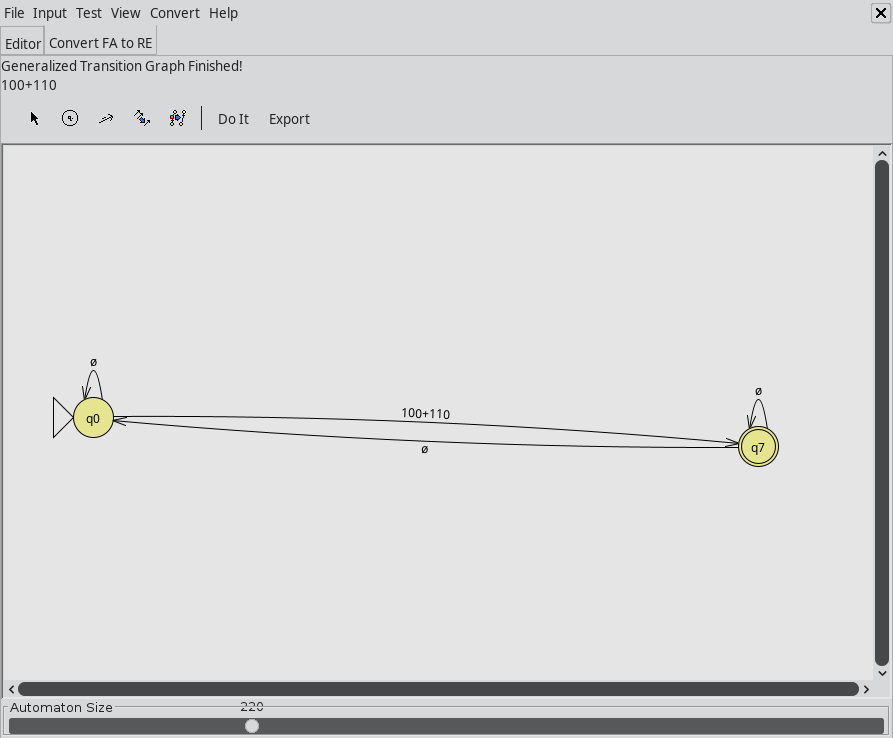
\includegraphics[scale=0.70]{jflap}
\caption{Resultado de conversión del autómata en jFlap.}
\end{center}
\end{figure}


\end{document}
